%%%%%%%%%%%%%%%%%%%%%%%%%%%%%%%%%%%%%%%%%
% Programming/Coding Assignment
% LaTeX Template
%
% This template has been downloaded from:
% http://www.latextemplates.com
%
% Original author:
% Ted Pavlic (http://www.tedpavlic.com)
%
% Note:
% The \lipsum[#] commands throughout this template generate dummy text
% to fill the template out. These commands should all be removed when 
% writing assignment content.
%
% This template uses a Perl script as an example snippet of code, most other
% languages are also usable. Configure them in the "CODE INCLUSION 
% CONFIGURATION" section.
%
%%%%%%%%%%%%%%%%%%%%%%%%%%%%%%%%%%%%%%%%%

%----------------------------------------------------------------------------------------
%	PACKAGES AND OTHER DOCUMENT CONFIGURATIONS
%----------------------------------------------------------------------------------------

\documentclass{article}

\usepackage{fancyhdr} % Required for custom headers
\usepackage{lastpage} % Required to determine the last page for the footer
\usepackage{extramarks} % Required for headers and footers
\usepackage[usenames,dvipsnames]{color} % Required for custom colors
\usepackage{graphicx} % Required to insert images
\usepackage{listings} % Required for insertion of code
\usepackage{courier} % Required for the courier font
\usepackage{lipsum} % Used for inserting dummy 'Lorem ipsum' text into the template
\usepackage{setspace}
\usepackage{color}
\usepackage{comment}
\usepackage{caption}

\usepackage{hyperref}
\usepackage{natbib}
\usepackage{underscore}

\hypersetup{
    colorlinks=true,
    linkcolor=blue,
    filecolor=magenta,      
    urlcolor=cyan,
    breaklinks=true
}

%\usepackage[]{algorithm2e}
\usepackage{pdfpages}




%For python inclusion (http://widerin.org/blog/syntax-highlighting-for-python-scripts-in-latex-documents)
\definecolor{Code}{rgb}{0,0,0}
\definecolor{Decorators}{rgb}{0.5,0.5,0.5}
\definecolor{Numbers}{rgb}{0.5,0,0}
\definecolor{MatchingBrackets}{rgb}{0.25,0.5,0.5}
\definecolor{Keywords}{rgb}{0,0,1}
\definecolor{self}{rgb}{0,0,0}
\definecolor{Strings}{rgb}{0,0.63,0}
\definecolor{Comments}{rgb}{0,0.63,1}
\definecolor{Backquotes}{rgb}{0,0,0}
\definecolor{Classname}{rgb}{0,0,0}
\definecolor{FunctionName}{rgb}{0,0,0}
\definecolor{Operators}{rgb}{0,0,0}
\definecolor{Background}{rgb}{0.98,0.98,0.98}

% Margins
\topmargin=-0.45in
\evensidemargin=0in
\oddsidemargin=0in
\textwidth=6.5in
\textheight=9.0in
\headsep=0.25in

\linespread{1.1} % Line spacing

% Set up the header and footer
\pagestyle{fancy}
\lhead{\hmwkAuthorName} % Top left header
%\chead{\hmwkClass\ (\hmwkClassInstructor\ \hmwkClassTime): \hmwkTitle} % Top center head
\chead{\hmwkClass\ (\hmwkClassInstructor): \hmwkTitle} % Top center head
\rhead{\firstxmark} % Top right header
\lfoot{\lastxmark} % Bottom left footer
\cfoot{} % Bottom center footer
\rfoot{Page\ \thepage\ of\ \protect\pageref{LastPage}} % Bottom right footer
\renewcommand\headrulewidth{0.4pt} % Size of the header rule
\renewcommand\footrulewidth{0.4pt} % Size of the footer rule

\setlength\parindent{0pt} % Removes all indentation from paragraphs

%----------------------------------------------------------------------------------------
%	CODE INCLUSION CONFIGURATION
%----------------------------------------------------------------------------------------

\definecolor{MyDarkGreen}{rgb}{0.0,0.4,0.0} % This is the color used for comments
\lstloadlanguages{Perl} % Load Perl syntax for listings, for a list of other languages supported see: ftp://ftp.tex.ac.uk/tex-archive/macros/latex/contrib/listings/listings.pdf
\lstset{language=Perl, % Use Perl in this example
        frame=single, % Single frame around code
        basicstyle=\small\ttfamily, % Use small true type font
        keywordstyle=[1]\color{Blue}\bf, % Perl functions bold and blue
        keywordstyle=[2]\color{Purple}, % Perl function arguments purple
        keywordstyle=[3]\color{Blue}\underbar, % Custom functions underlined and blue
        identifierstyle=, % Nothing special about identifiers                                         
        commentstyle=\usefont{T1}{pcr}{m}{sl}\color{MyDarkGreen}\small, % Comments small dark green courier font
        stringstyle=\color{Purple}, % Strings are purple
        showstringspaces=false, % Don't put marks in string spaces
        tabsize=5, % 5 spaces per tab
        %
        % Put standard Perl functions not included in the default language here
        morekeywords={rand},
        %
        % Put Perl function parameters here
        morekeywords=[2]{on, off, interp},
        %
        % Put user defined functions here
        morekeywords=[3]{test},
       	%
        morecomment=[l][\color{Blue}]{...}, % Line continuation (...) like blue comment
        numbers=left, % Line numbers on left
        firstnumber=1, % Line numbers start with line 1
        numberstyle=\tiny\color{Blue}, % Line numbers are blue and small
        stepnumber=5 % Line numbers go in steps of 5
}

% Creates a new command to include a perl script, the first parameter is the filename of the script (without .pl), the second parameter is the caption
\newcommand{\perlscript}[2]{
\begin{itemize}
\item[]\lstinputlisting[caption=#2,label=#1]{#1.pl}
\end{itemize}
}


%----------------------------------------------------------------------------------------
%	DOCUMENT STRUCTURE COMMANDS
%	Skip this unless you know what you're doing
%----------------------------------------------------------------------------------------

% Header and footer for when a page split occurs within a problem environment
\newcommand{\enterProblemHeader}[1]{
\nobreak\extramarks{#1}{#1 continued on next page\ldots}\nobreak
\nobreak\extramarks{#1 (continued)}{#1 continued on next page\ldots}\nobreak
}

% Header and footer for when a page split occurs between problem environments
\newcommand{\exitProblemHeader}[1]{
\nobreak\extramarks{#1 (continued)}{#1 continued on next page\ldots}\nobreak
\nobreak\extramarks{#1}{}\nobreak
}

\setcounter{secnumdepth}{0} % Removes default section numbers
\newcounter{homeworkProblemCounter} % Creates a counter to keep track of the number of problems

\newcommand{\homeworkProblemName}{}
\newenvironment{homeworkProblem}[1][Problem \arabic{homeworkProblemCounter}]{ % Makes a new environment called homeworkProblem which takes 1 argument (custom name) but the default is "Problem #"
\stepcounter{homeworkProblemCounter} % Increase counter for number of problems
\renewcommand{\homeworkProblemName}{#1} % Assign \homeworkProblemName the name of the problem
\section{\homeworkProblemName} % Make a section in the document with the custom problem count
\enterProblemHeader{\homeworkProblemName} % Header and footer within the environment
}{
\exitProblemHeader{\homeworkProblemName} % Header and footer after the environment
}

\newcommand{\problemAnswer}[1]{ % Defines the problem answer command with the content as the only argument
\noindent\framebox[\columnwidth][c]{\begin{minipage}{0.98\columnwidth}#1\end{minipage}} % Makes the box around the problem answer and puts the content inside
}

\newcommand{\homeworkSectionName}{}
\newenvironment{homeworkSection}[1]{ % New environment for sections within homework problems, takes 1 argument - the name of the section
\renewcommand{\homeworkSectionName}{#1} % Assign \homeworkSectionName to the name of the section from the environment argument
\subsection{\homeworkSectionName} % Make a subsection with the custom name of the subsection
\enterProblemHeader{\homeworkProblemName\ [\homeworkSectionName]} % Header and footer within the environment
}{
\enterProblemHeader{\homeworkProblemName} % Header and footer after the environment
}

%----------------------------------------------------------------------------------------
%	NAME AND CLASS SECTION
%----------------------------------------------------------------------------------------

\newcommand{\hmwkTitle}{Assignment\ \#4 } % Assignment title
%\newcommand{\hmwkDueDate}{Monday,\ January\ 1,\ 2012} % Due date
\newcommand{\hmwkClass}{Introduction to Web Science} % Course/class
%\newcommand{\hmwkClassTime}{10:30am} % Class/lecture time
\newcommand{\hmwkClassInstructor}{Dr. Nelson} % Teacher/lecturer
\newcommand{\hmwkAuthorName}{Alexander Nwala} % Your name

%----------------------------------------------------------------------------------------
%	TITLE PAGE
%----------------------------------------------------------------------------------------

\title{
\vspace{2in}
\textmd{\textbf{\hmwkClass:\ \hmwkTitle}}\\
%\normalsize\vspace{0.1in}\small{Due\ on\ \hmwkDueDate}\\
%\vspace{0.1in}\large{\textit{\hmwkClassInstructor\ \hmwkClassTime}}
\vspace{0.1in}\large{\textit{\hmwkClassInstructor}}
\vspace{3in}
}

\author{\textbf{\hmwkAuthorName}}
\date{Thursday, October 9, 2014} % Insert date here if you want it to appear below your name

%----------------------------------------------------------------------------------------

\begin{document}

\maketitle



%----------------------------------------------------------------------------------------
%	TABLE OF CONTENTS
%----------------------------------------------------------------------------------------

%\setcounter{tocdepth}{1} % Uncomment this line if you don't want subsections listed in the ToC

\newpage
\tableofcontents
\newpage

%----------------------------------------------------------------------------------------
%	PROBLEM 1
%----------------------------------------------------------------------------------------

% To have just one problem per page, simply put a \clearpage after each problem

\begin{homeworkProblem}

From your list of 1000 links, choose 100 and extract all of the
links from those 100 pages to other pages.  We're looking for user 
navigable links, that is in the form of: 

\begin{verbatim}
<A href="foo">bar</a>
\end{verbatim}

We're not looking for embedded images, scripts, \textless link\textgreater elements,
etc.  You'll probably want to use BeautifulSoup for this.

For each URI, create a text file of all of the outbound links from
that page to other URIs (use any syntax that is easy for you).  For
example:

\begin{verbatim}
site: 
    http://www.cs.odu.edu/~mln/    
links:
    http://www.cs.odu.edu/
    http://www.odu.edu/
    http://www.cs.odu.edu/~mln/research/
    http://www.cs.odu.edu/~mln/pubs/
    http://ws-dl.blogspot.com/
    http://ws-dl.blogspot.com/2013/09/2013-09-09-ms-thesis-http-mailbox.html
    etc.
\end{verbatim}

Upload these 100 files to github (they don't have to be in your report).


%\lstinputlisting[breaklines=true, caption=Curl Demo]{"/home/anwala/CS 895/Assignment 1/problem1_curlDemonstration.py"}
%\lstinputlisting[breaklines=true, caption=Hash function; extract HTML funtion; and strip HTML tags function]{hashExtractProcessHTMlSnippet.py}


\begin{comment}
\begin{figure}
    \caption{curlDemoOutput}
    \begin{center}
        \includegraphics{curlDemo} % Example image
    \end{center}
\end{figure}
\end{comment}

%\problemAnswer
%{
    \begin{verbatim}\end{verbatim}
    \textbf{SOLUTION 1}\\

    The solution for this problem is outlined by the following steps:
    \begin{enumerate}

    \item \textbf{Download links:}  Given inputs derived from a file (\textbf{URIs.txt}) containing 1000 unique URIs downloaded from twitter, all links from all the URIs were extracted using Beautiful soup (Listing 1.) and stored in individual files as well as a master file of format:
    \begin{verbatim}
        parentURI0
            childURI0
            childURI1
        parentURI1
            childURI0
            childURI1
        .
        .
        .
        parentURI(n-1)
            childURI0
            childURI1

        In this representaion, childURI(n) was extracted from the 
        parentURI(n)
    \end{verbatim}

    \lstinputlisting[breaklines=true, caption=Extract links]{extractLinksSnippet.py}

    \item \textbf{Select 100 parent/child URI files:} This was achieved through the following selection criteria:
    \begin{verbatim}
        a. Expand shortened URIs (Listing 2)
        b. To limit the size of the graph, if a parent has over 
           50 child links, select 50 or 25
        c. Given a collection of child links, select those that offer 
           the most variety (those from a different domain than already
           selected)
    \end{verbatim}
    The final set of 100 parent/child URIs were stored in a master file (\textbf{100\_parentChildLinks.txt}).
    Finally, from this file, 100 individual parent/child files were written into the folder \textbf{100Links}
    \lstinputlisting[breaklines=true, caption=Expand short URIs]{expandURISnippet.py}

    \end{enumerate}
%}

\end{homeworkProblem}

%----------------------------------------------------------------------------------------
%	PROBLEM 2
%----------------------------------------------------------------------------------------

\begin{homeworkProblem}
Using these 100 files, create a single GraphViz ``dot'' file of
the resulting graph.  Learn about dot at:

\begin{verbatim}
Examples:
    http://www.graphviz.org/content/unix
    http://www.graphviz.org/Gallery/directed/unix.gv.txt

Manual:
    http://www.graphviz.org/Documentation/dotguide.pdf

Reference:
    http://www.graphviz.org/content/dot-language
    http://www.graphviz.org/Documentation.php

Note: you'll have to put explicit labels on the graph, see:
   https://gephi.org/users/supported-graph-formats/graphviz-dot-format/
   (note: actually, I'll allow any of the formats listed here:
   https://gephi.org/users/supported-graph-formats/
   but ``dot'' is probably the simplest.)
\end{verbatim}

\begin{verbatim}\end{verbatim}
\textbf{SOLUTION 2}\\

Given input from the master file of 100 URIs of parent/child links (\textbf{100\_parentChildLinks.txt}), 
due to Listing 3, the input file was converted into a dot file.

\begin{verbatim}
    The file parentChildURIs.dot contains the complete graph
\end{verbatim}

\lstinputlisting[breaklines=true, caption=Convert to dot file]{convertToDotFileSnippet.py}

In order to facilitate visualization, the following label shortening scheme was applied:
\begin{enumerate}
    \item Remove the scheme (http://, https://, etc)
    \item Remove www.
    \item Remove path
    \item remove tld (.com, .edu, .org, etc)
\end{enumerate}


\begin{comment}
\begin{figure}
\caption{Uris distribution}
\begin{center}
    %\includegraphics{/home/anwala/CS895/Assignment2/urisDistribution.png} % Example image
    %\includepdf[pages={1},width=\textwidth,scale=0.5]{/home/anwala/CS895/Assignment2/Rplots.pdf}
\end{center}
\end{figure}
\end{comment}

\end{homeworkProblem}

%----------------------------------------------------------------------------------------
%   PROBLEM 3
%----------------------------------------------------------------------------------------
\begin{homeworkProblem}

Download and install Gephi: \url{https://gephi.org/}

Load the dot file created in \#2 and use Gephi to:

\begin{verbatim}
- visualize the graph (you'll have to turn on labels)
- calculate HITS and PageRank
- avg degree
- network diameter
- connected components
\end{verbatim}

Put the resulting graphs in your report.

You might need to choose the 100 sites with an eye toward
creating a graph with at least one component that is nicely
connected.  You can probably do this by selecting some portion
of your links (e.g., 25, 50) from the same site.  

\begin{verbatim} \end{verbatim}
\textbf{SOLUTION 3}\\

In order to better visualize the graph, I chose the Fruchterman-Reingold algorithm\cite{FR} to render the graph.
This method belongs to a class of force-directed algorithm which help reduce edge crossing.\\

Furthermore, in order to explore the connectedness of the graph I chose the YiFan Hu proportional algorithm\cite{YFH} (also a force-directed algorithm) to visualize the 
graph. From Figure 3, we can see the graph has many isolated partitions (hub/spoke) and a couple of links exist between these.\\

In addition, to add another dimension to the graph, the nodes are labelled and colored according to the
respective labels.\\

The resultant directed graph contains 781 nodes adn 801 edges. In Figures 1-3, common colors (node/edge) represent labels with common names. Note that due to the label shortening scheme, multiple nodes have the same labels, eventhough they have different full names.\\

%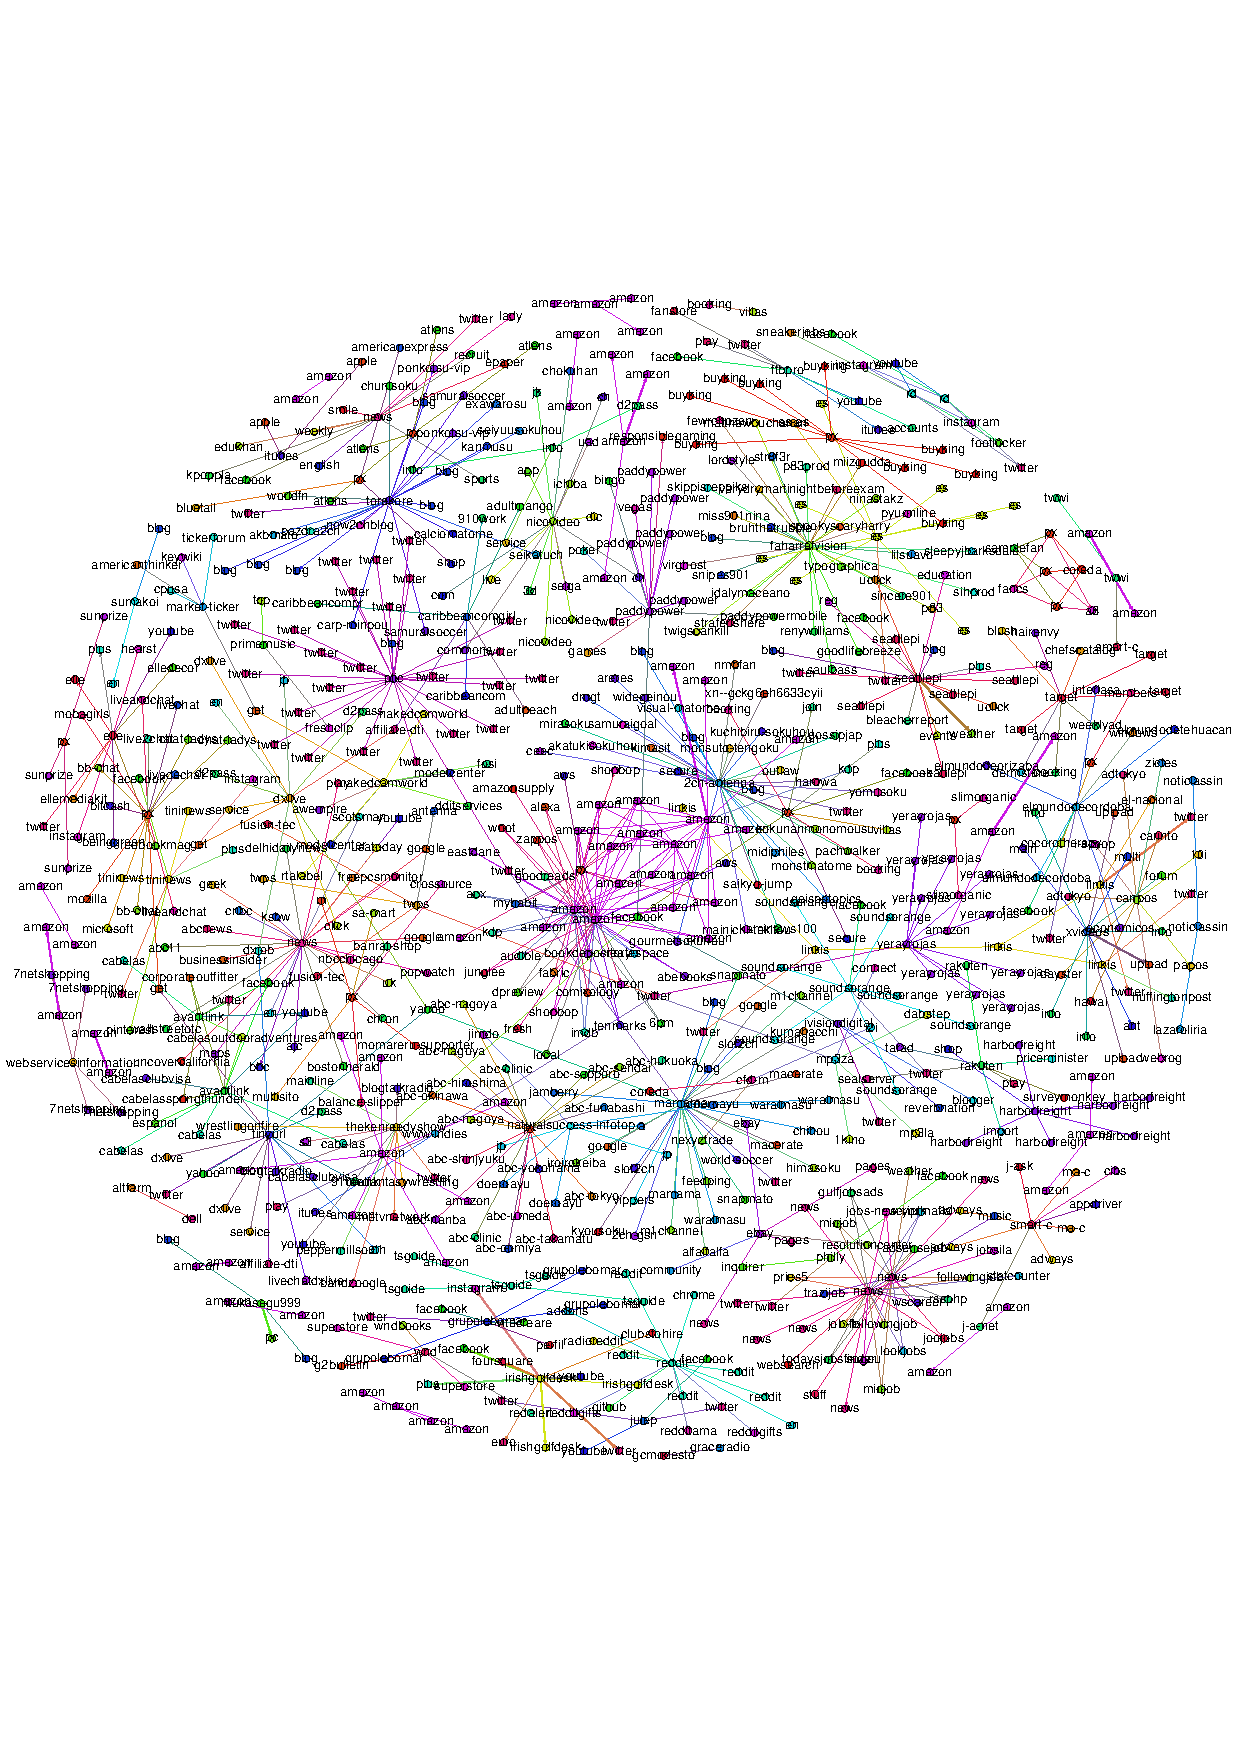
\includepdf[pages={1},width=\textwidth,scale=0.5]{allNodes.pdf}
\begin{figure}
\caption{All nodes, Fruchterman Reingold visualization algorithm}
 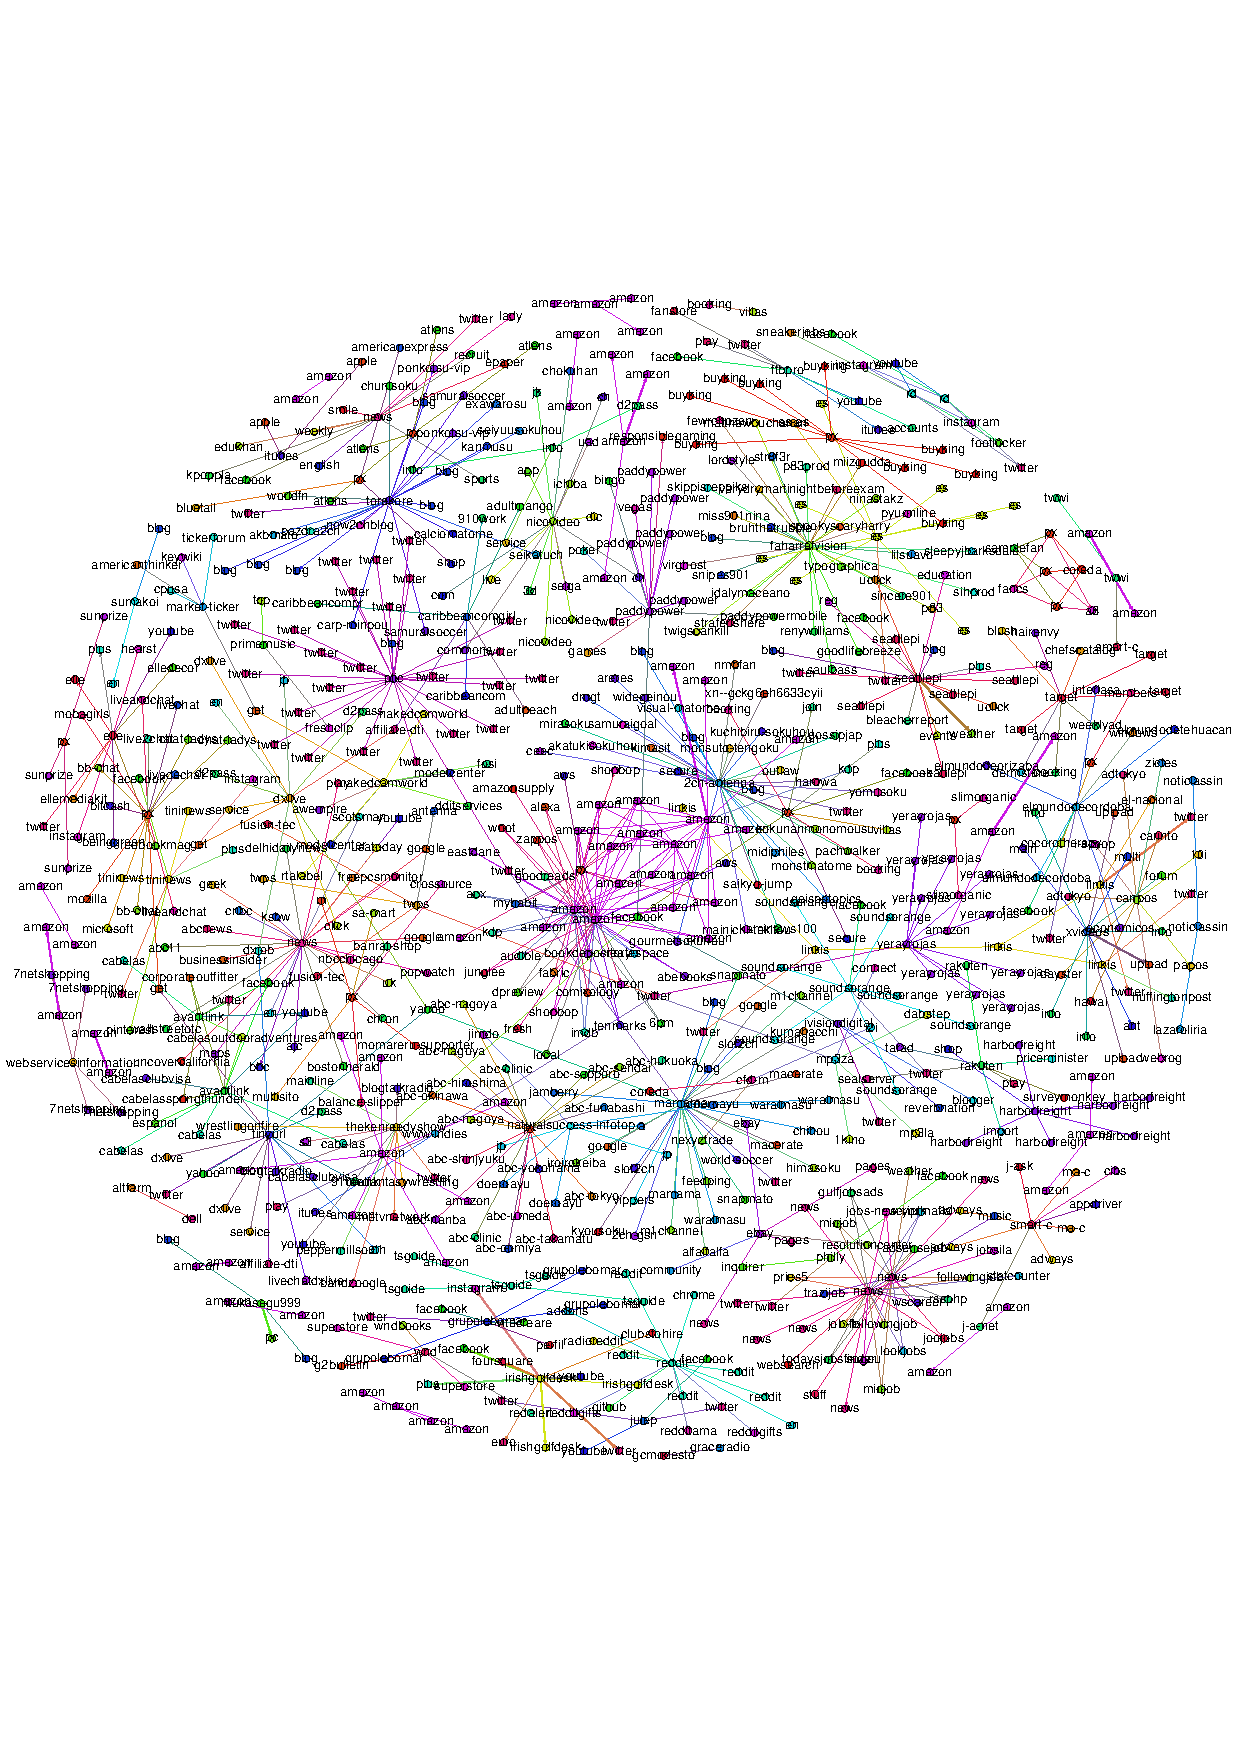
\includegraphics[width=\textwidth,scale=0.5]{allNodes.pdf}
\end{figure}

\begin{figure}
\caption{All nodes with boxed labels, Fruchterman Reingold visualization algorithm}
 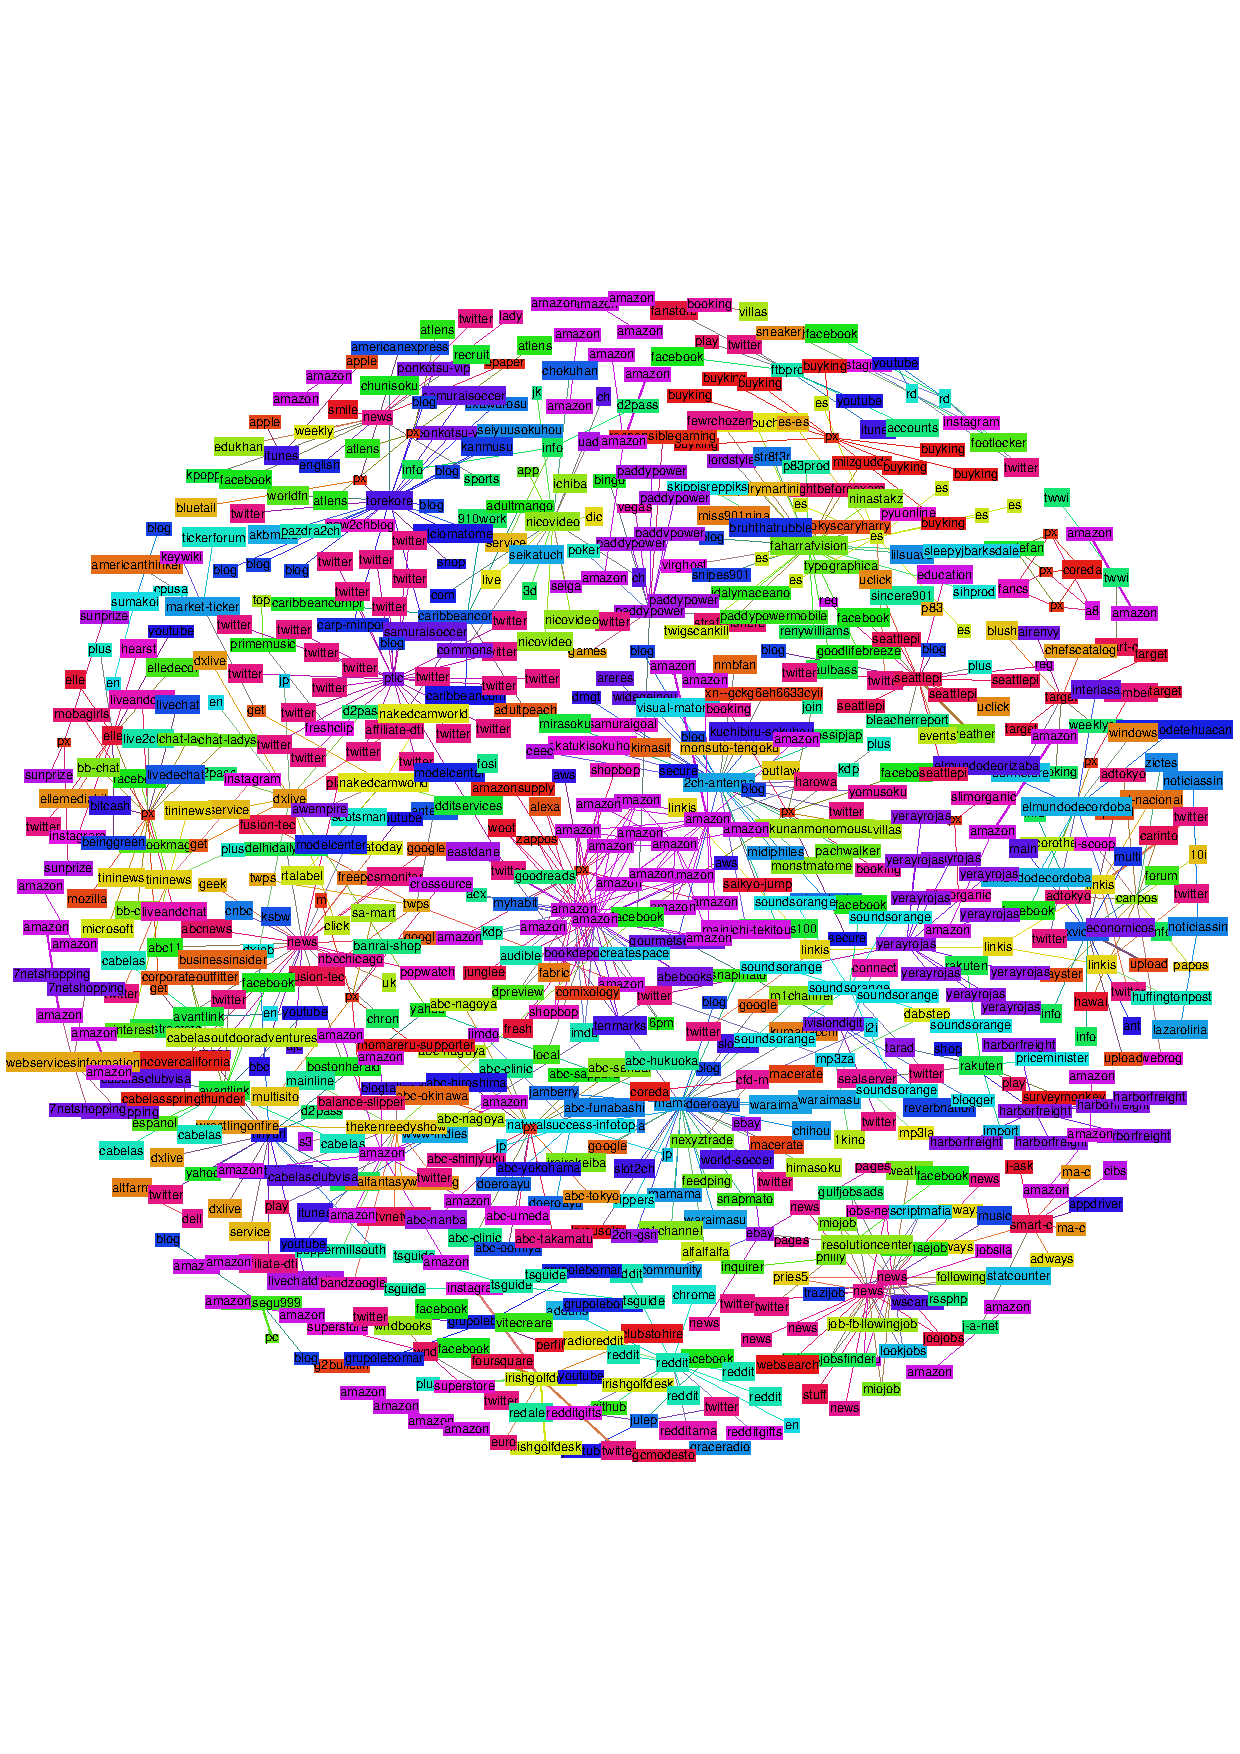
\includegraphics[width=\textwidth,scale=0.5]{allNodes2.pdf}
\end{figure}

\begin{figure}
\caption{All nodes, Yifan Hu Proportional visualization algorithm}
 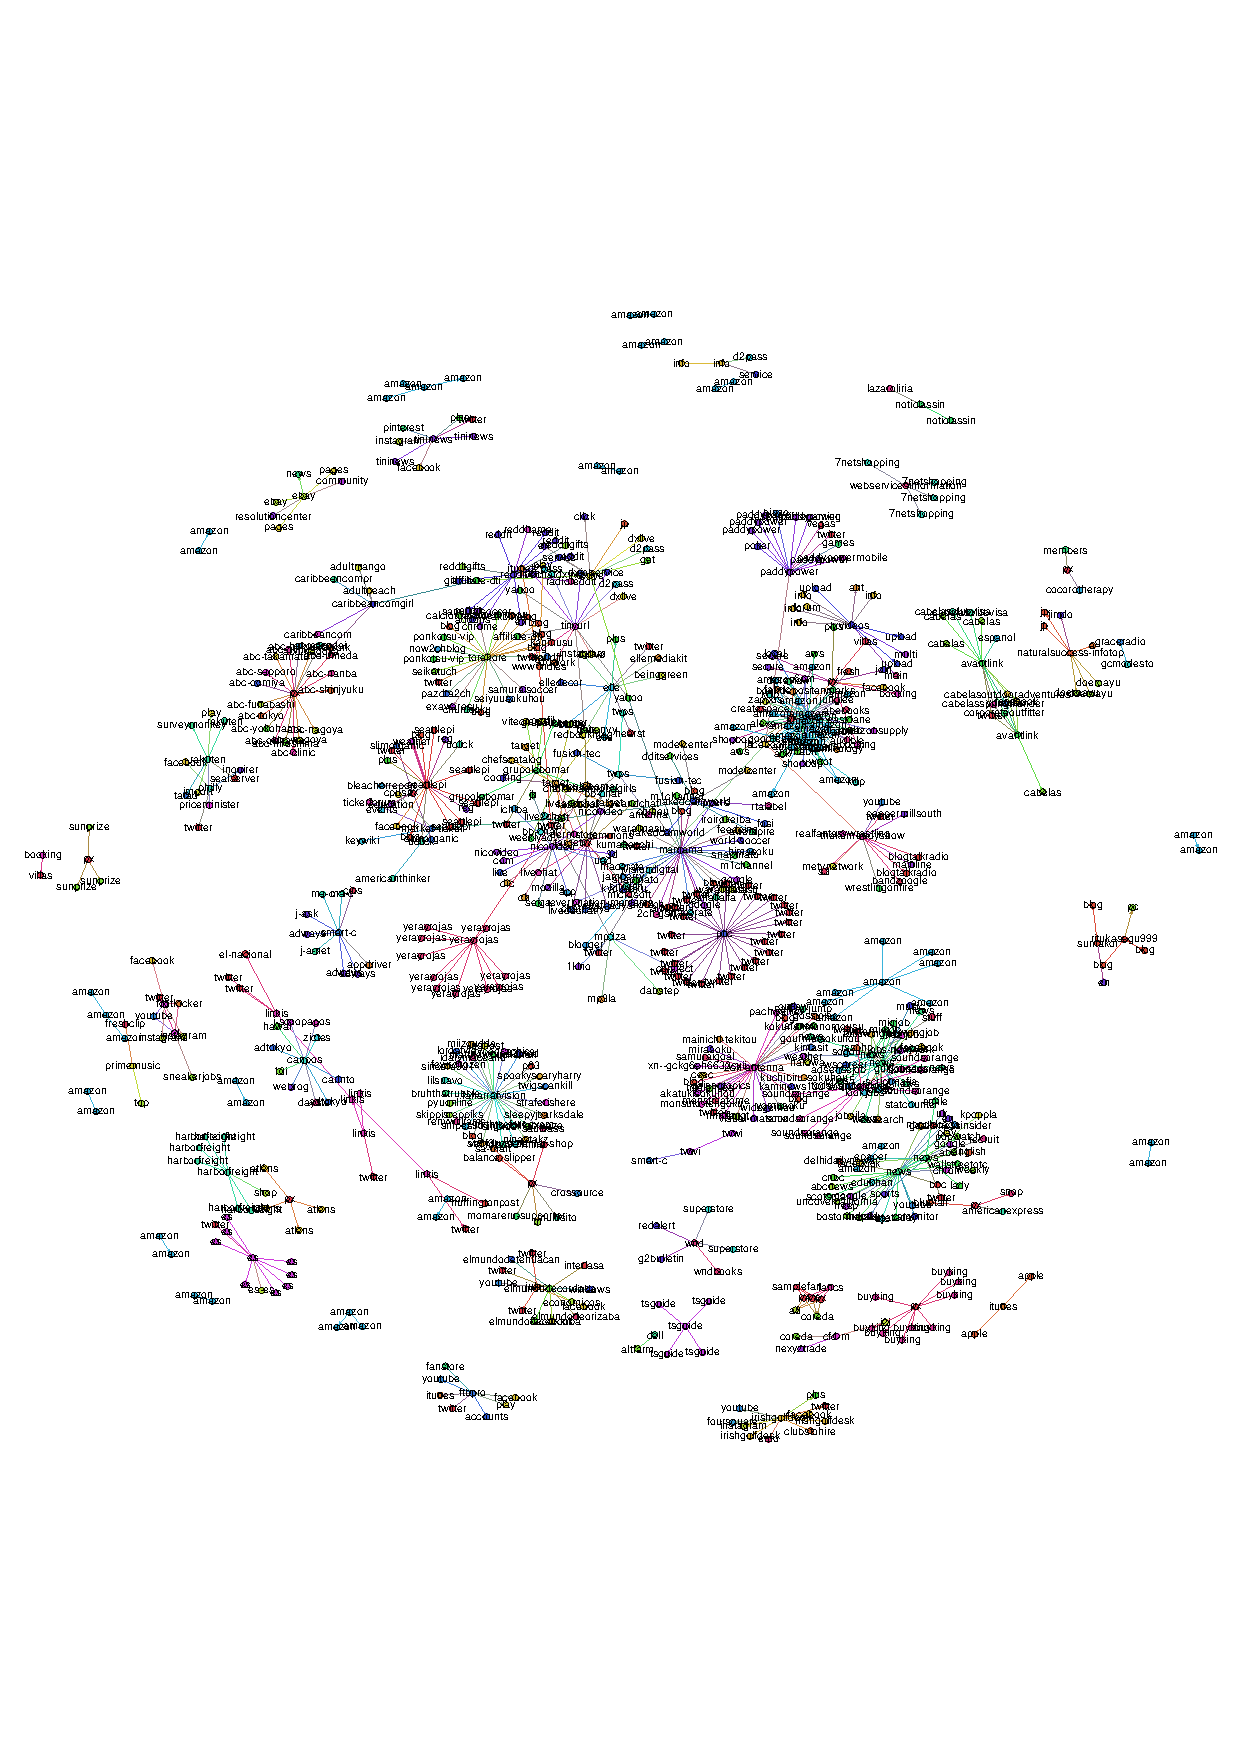
\includegraphics[width=\textwidth,scale=0.5]{allNodesYuFanHu.pdf}
\end{figure}

\begin{figure}
\caption{Partitioning based on node importance}
 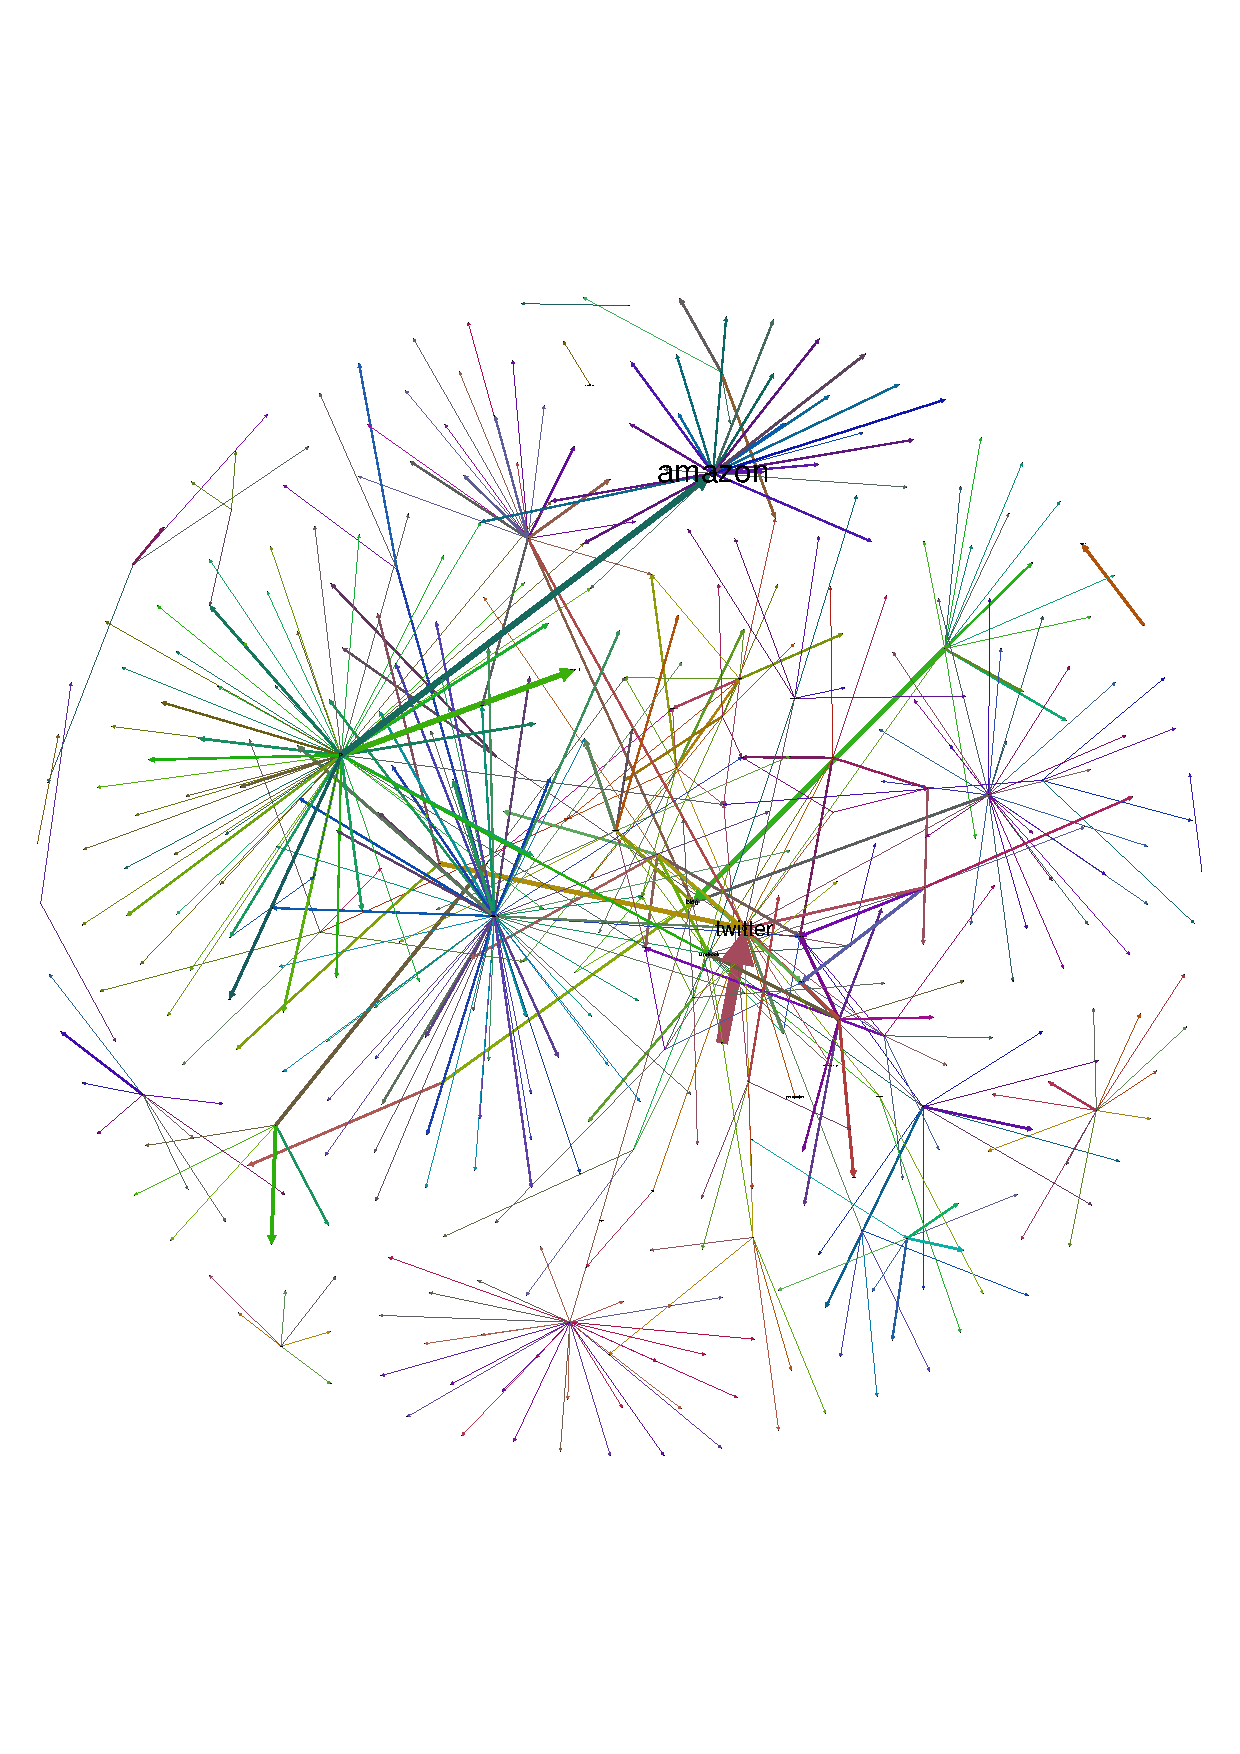
\includegraphics[width=\textwidth,scale=0.5]{importantNodes.pdf}
\end{figure}

From Figures 1 and 2, since the links were extracted from random site, the graph tends has many 
isolated partitions: this is reflected by the number of weakly connected components.\\

The following parameters were derived from the graph:

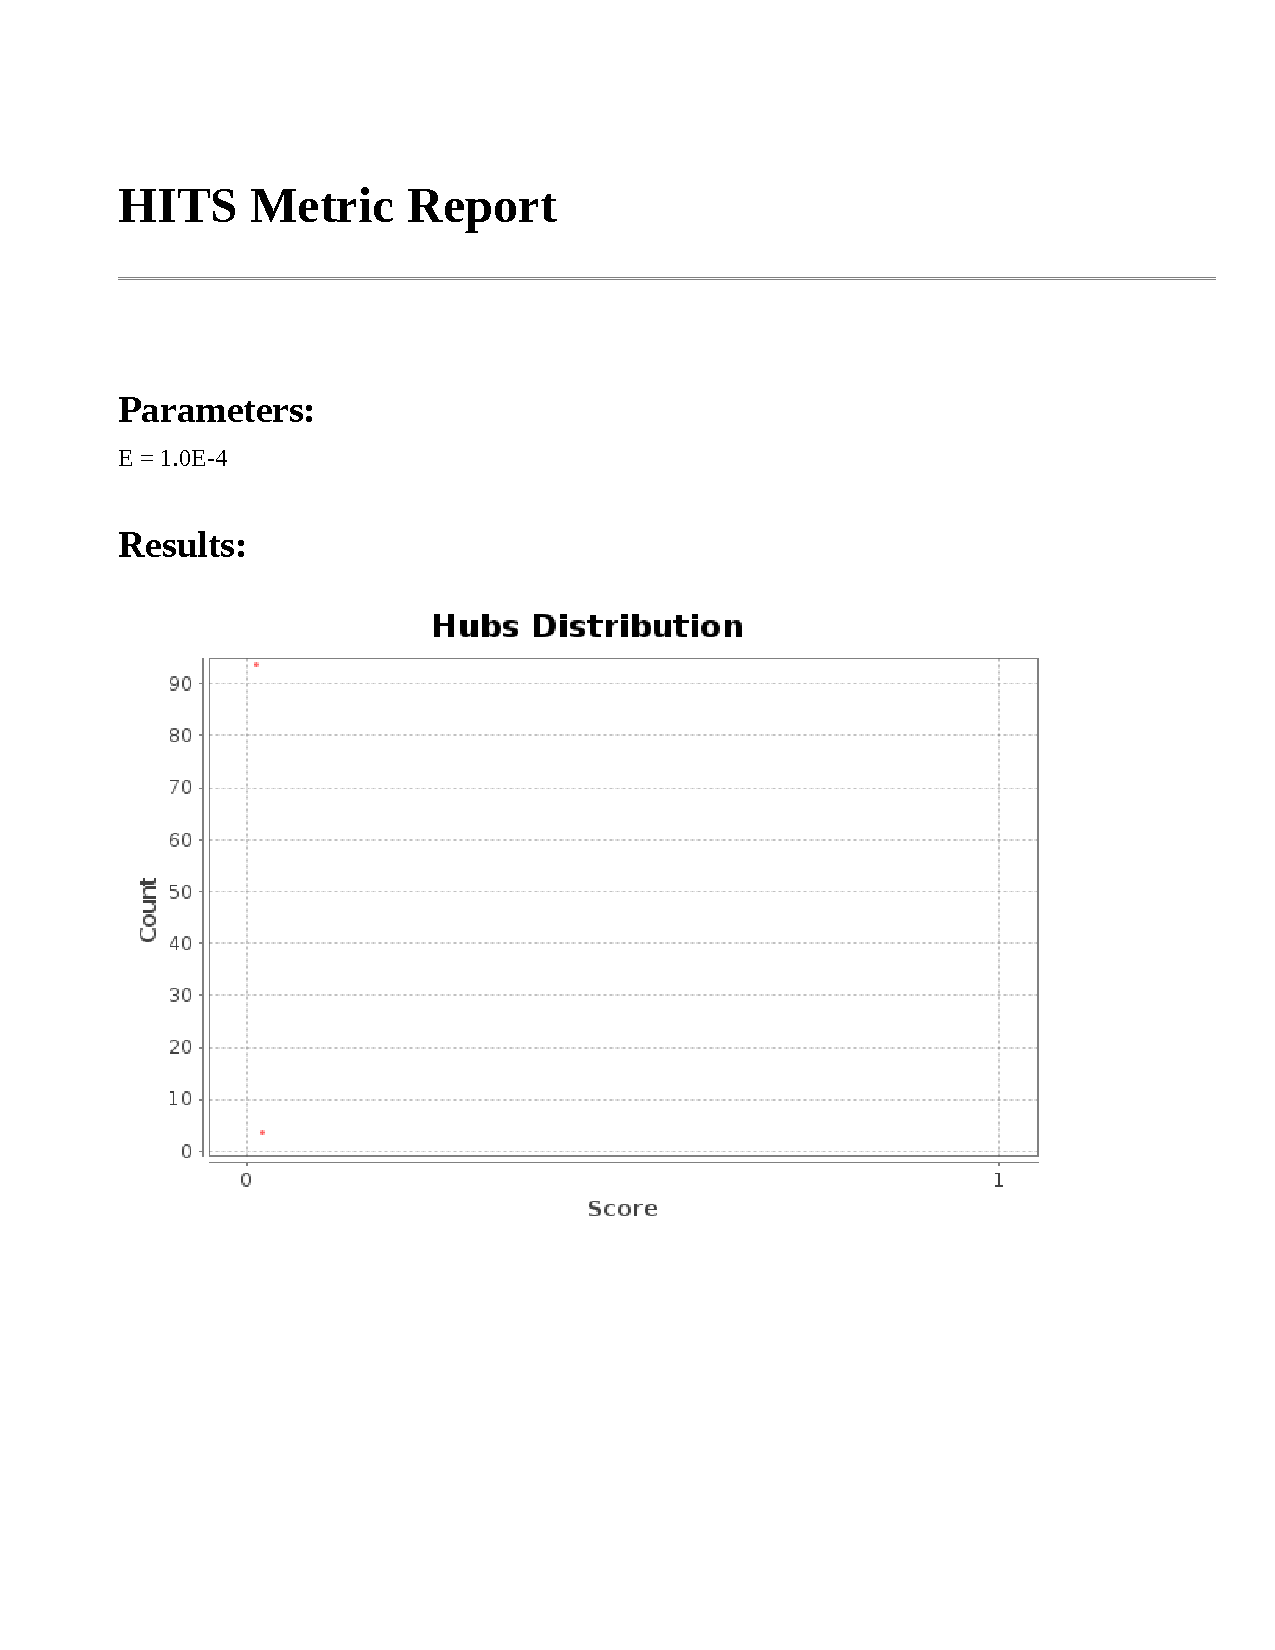
\includepdf[pages={1-}, width=\textwidth,scale=0.5]{HITSReport.pdf}
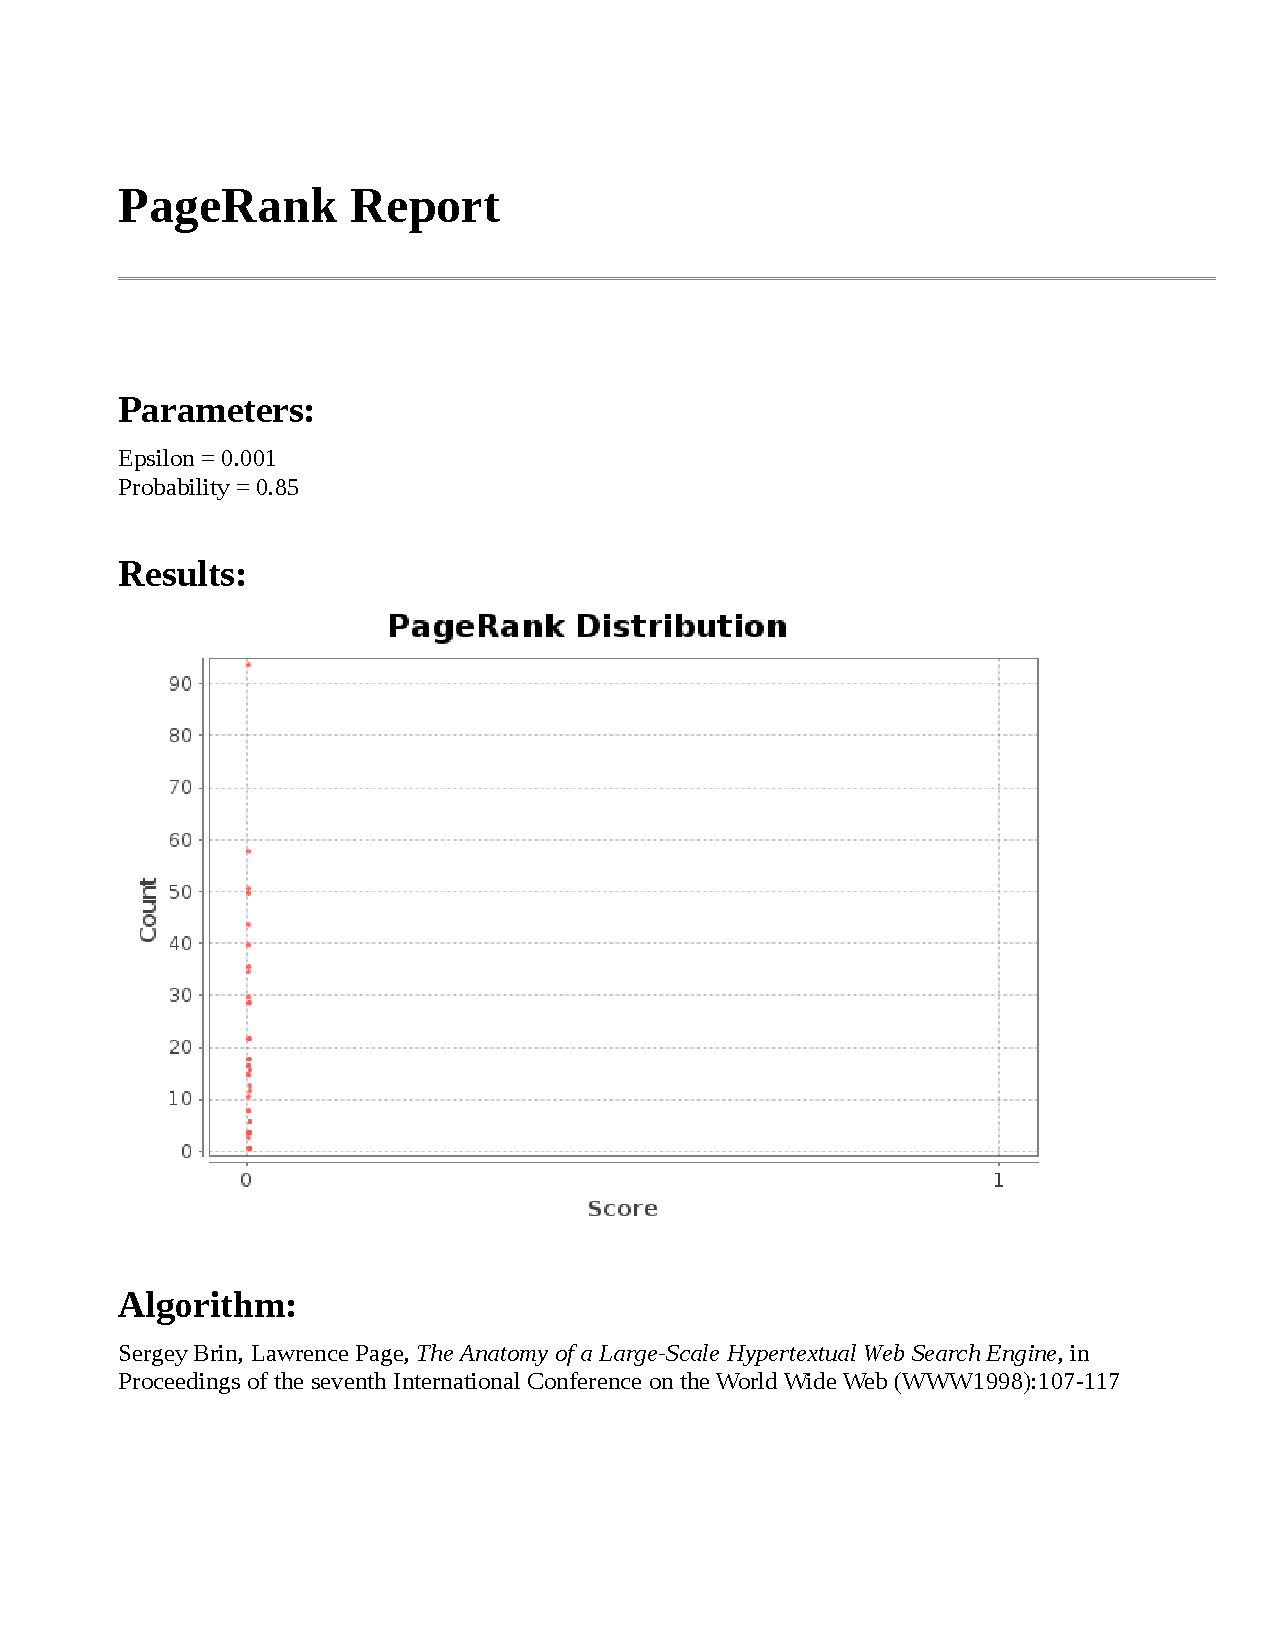
\includepdf[pages={1-}, width=\textwidth,scale=0.5]{pageRankReport.pdf}
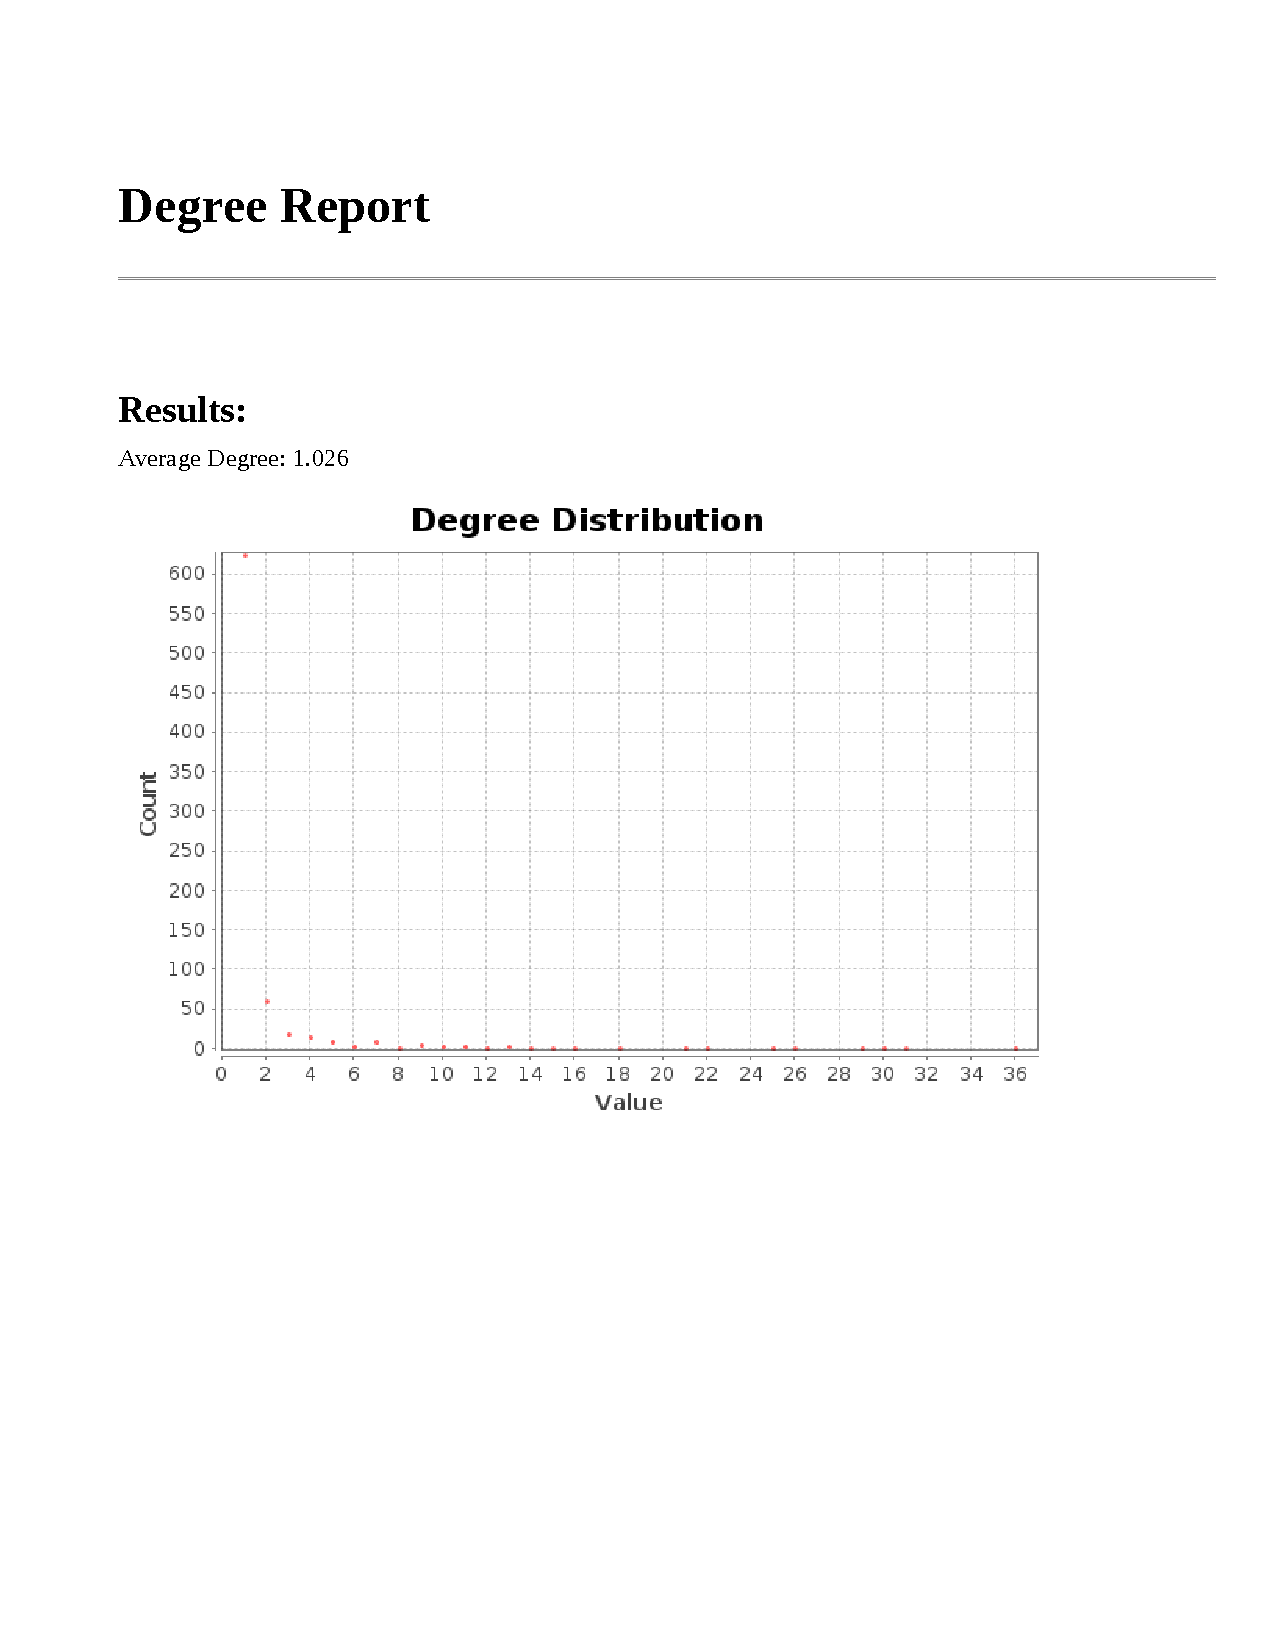
\includepdf[pages={1-}, width=\textwidth,scale=0.5]{averageDegreeReport.pdf}
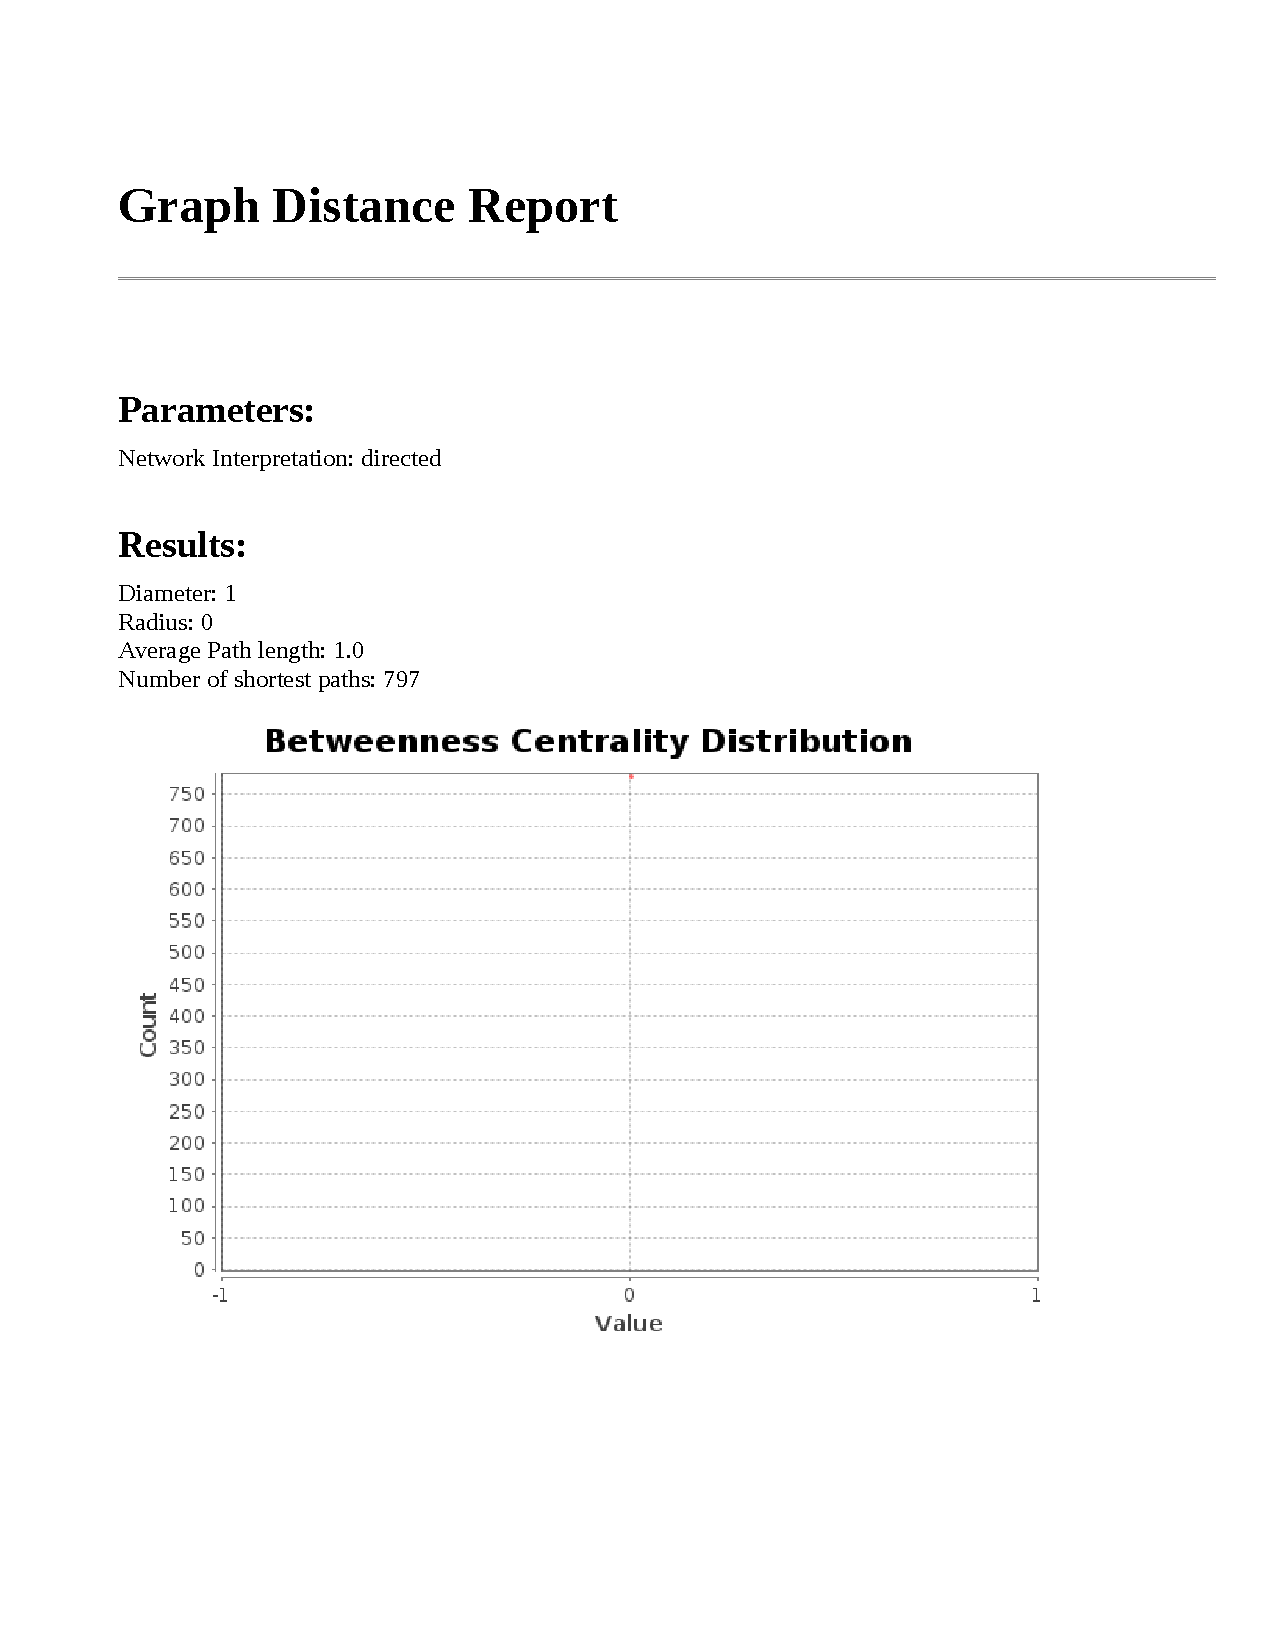
\includepdf[pages={1-}, width=\textwidth,scale=0.5]{networkDiameterReport.pdf}
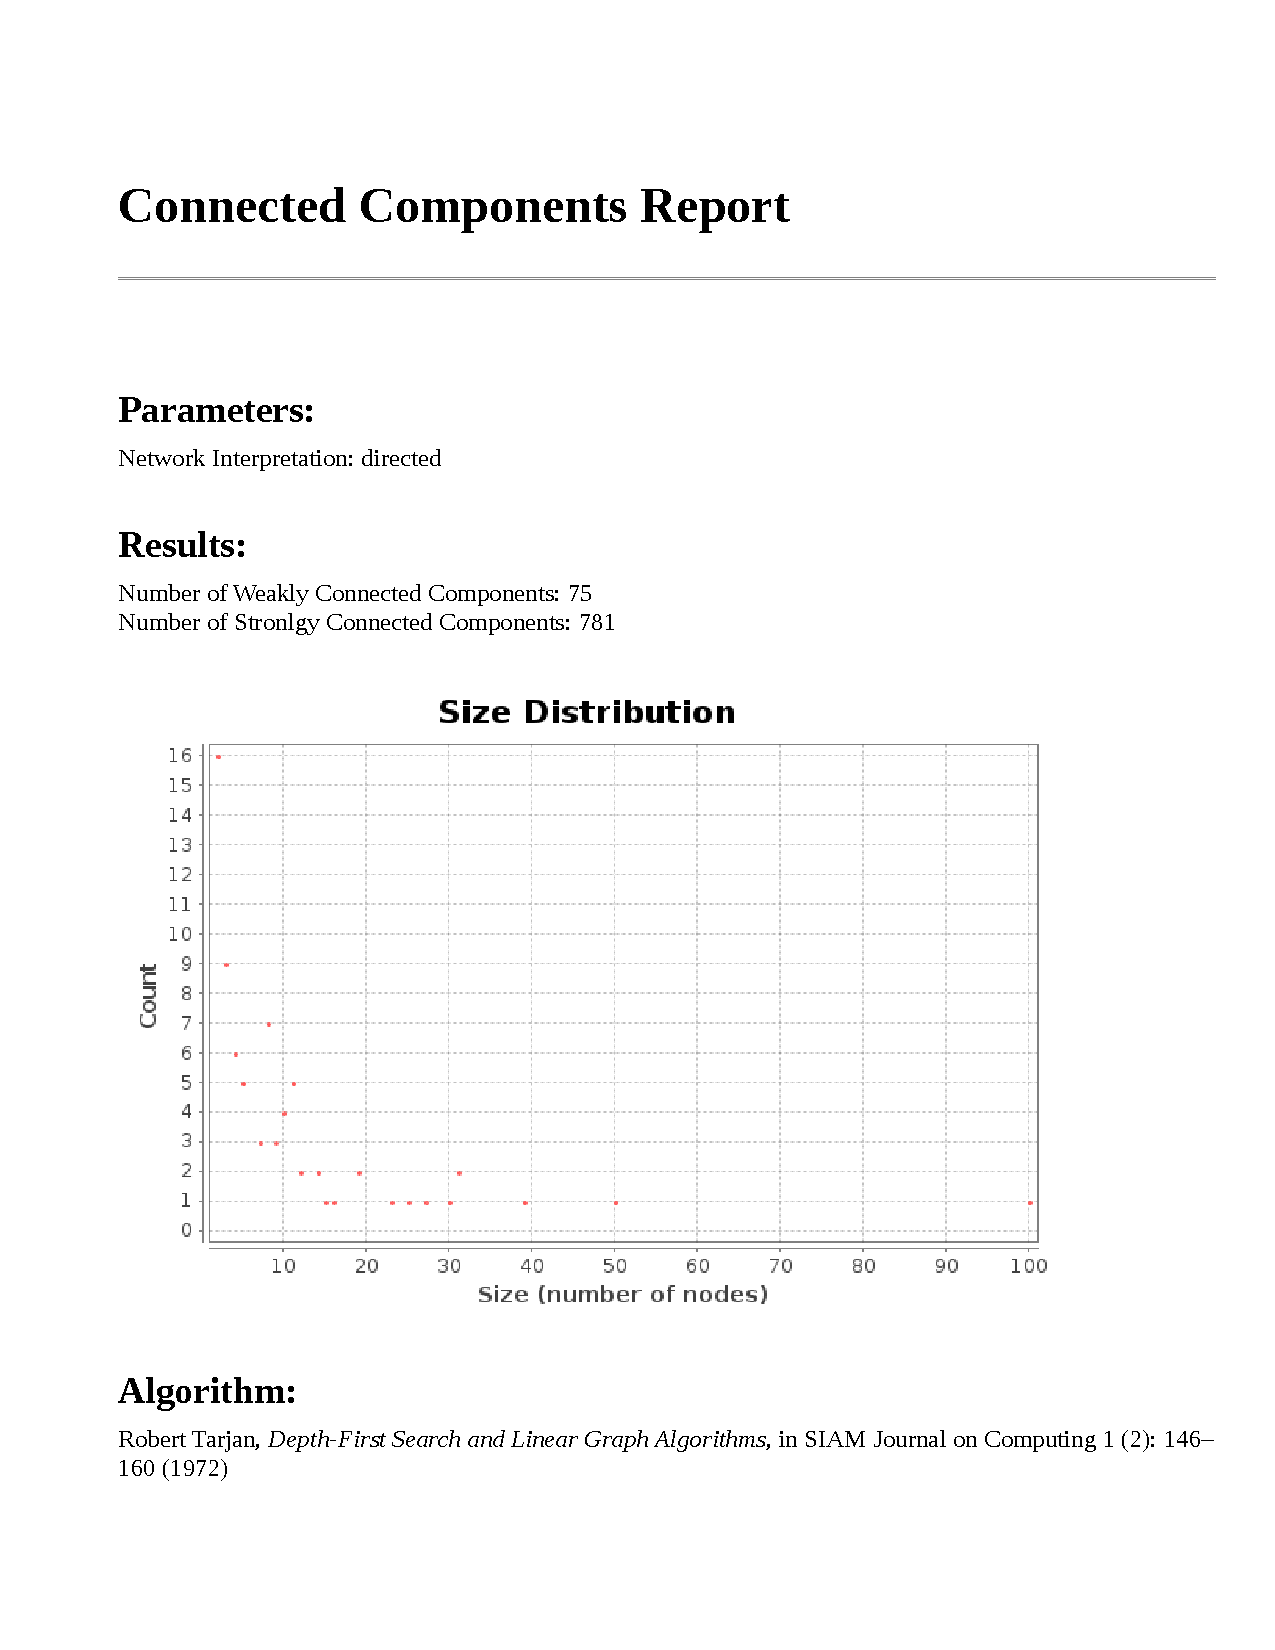
\includepdf[pages={1-}, width=\textwidth,scale=0.5]{connectedComponentReport.pdf}

\textbf{Summary:}
The number of strongly connected components given by Gephi is incorrect since it is clear the graph is made up of multiple 
isolated partitions.\\

Even though the graph has many disconnected partitions due to the random nature of the data, we can see that the nodes with label ``amazon'' and ``twitter'' are very important since they are linked by other partitions regardless of the random nature of the data (Figure 4).

\end{homeworkProblem}
\begin{verbatim}\end{verbatim}







\bibliographystyle{plain}
\bibliography{A4bibFile}

%----------------------------------------------------------------------------------------

\end{document}